\subchapter{Module development environment}{Objective: Setup an NFS
  based kernel module development environment}

After this lab, you will be able to:
\begin{itemize}

\item Cross-compile a kernel for the ARM platform

\item Boot this kernel on an NFS root filesystem, which is somewhere
on your development workstation\footnote{NFS root filesystems are
particularly useful to compile modules on your host, and make them
directly visible on the target. You longer have to update the root
filesystem by hand and transfer it to the target (requiring a shutdown
and reboot).}

\end{itemize}

\section{Lab implementation}

While developing a kernel module, the developer wants to change the
source code, compile and test the new kernel module very
frequently. While writing and compiling the kernel module is done the
development workstation, the test of the kernel module usually has to
be done on the target, since it might interact with hardware specific
to the target.

However, flashing the root filesystem on the target for every test is
time-consuming and would use the flash chip needlessly.

Fortunately, it is possible to set up networking between the
development workstation and the target. Then, workstation files can be
accessed through the network by the target, using NFS.

\begin{center}
\includegraphics[width=\textwidth]{labs/kernel-module-environment/host-vs-target.pdf}
\end{center}

\section{Setup}

Stay in the \code{/home/<user>/felabs/linux/modules} directory.

Install packages needed for this lab:

\begin{verbatim}
sudo apt-get install libqt4-dev g++ u-boot-tools
\end{verbatim}

\code{libqt4-dev} and \code{g++} are needed for \code{make xconfig}.
\code{u-boot-tools} is needed to build the \code{uImage} file for
U-boot (\code{mkimage} utility).

\section{Cross-compiling toolchain setup}

We are going to install a cross-compiling toolchain from
Linaro\footnote{Note that Linaro toolchains by default generate code
for the \code{armv7} instruction set, while our AT91 CPU only supports
\code{armv5}. This is not a problem, as the kernel \code{Makefile} will
invoke the cross-compiler with the right instruction set settings.}, a
very popular source for ARM toolchains (amongst other useful resources
for Linux on ARM).

\begin{verbatim}
sudo apt-get install gcc-arm-linux-gnueabi
\end{verbatim}

Now find out the path and name of the cross-compiler executable by looking at the contents of the package:

\begin{verbatim}
dpkg -L gcc-arm-linux-gnueabi
\end{verbatim}

\section{Kernel configuration}

Set the \code{ARCH} and \code{CROSS_COMPILE} definitions for the \code{arm}
platform and to use your cross-compiler.

Configure this kernel with the ready-made configuration for boards
with the AT91SAM9263 CPU.

Make sure that this configuration has \code{CONFIG_ROOT_NFS=y} (support
booting on an NFS exported root directory).

Compile your kernel and generate the \code{uImage} kernel image that U-boot
needs (the U-boot bootloader needs the kernel \code{zImage} file to be
encapsulated in a special container and the kernel \code{Makefile} can
generate this container for you by running the mkimage tool found in
the \code{uboot-mkimage} package):

\begin{verbatim}
make uImage
\end{verbatim}

\section{Setting up the NFS server}

Install the NFS server by installing the \code{nfs-kernel-server}
package. Once installed, edit the \code{/etc/exports} file as
\code{root} to add the following lines, assuming that the IP address
of your board will be \code{192.168.0.100}:

\scriptsize
\begin{verbatim}
/home/<user>/felabs/linux/modules/nfsroot 192.168.0.100(rw,no_root_squash,no_subtree_check)
/home/<user>/felabs/linux/character/nfsroot 192.168.0.100(rw,no_root_squash,no_subtree_check)
/home/<user>/felabs/linux/debugging/nfsroot 192.168.0.100(rw,no_root_squash,no_subtree_check)
\end{verbatim}
\normalsize

Then, restart the NFS server:

\begin{verbatim}
sudo /etc/init.d/nfs-kernel-server restart
\end{verbatim}

If there is any error message, this usually means that there was a
syntax error in the \code{/etc/exports} file. Don't proceed until these
errors disappear.

\section{Setting up serial communication with the board}

Plug the Calao board on your computer using its USB-A connector. When
plugged-in, a new serial ports should appear: \code{/dev/ttyUSB0}.
You can also see this device appear by looking at the output of \code{dmesg}.

To communicate with the board through the serial port, install a serial communication program, such as \code{picocom}:

\begin{verbatim}
sudo apt-get install picocom
\end{verbatim}

Run \code{picocom -b 115200 /dev/ttyUSB0}, to start a serial
communication on \code{/dev/ttyUSB0}, with a baudrate of \code{115200}. If
you wish to exit \code{picocom}, press \code{[Ctrl][a]} followed by
\code{[Ctrl][x]}.

You should now see the U-Boot prompt:
\begin{verbatim}
U-Boot>
\end{verbatim}

You may need to reset the board (using the tiny reset button close to
the USB host connectors).

You can now use U-Boot. Run the \code{help} command to see the available
commands.

\section{Setting up Ethernet communication}

The kernel image will be transferred to the board using the TFTP
protocol, which works on top of an Ethernet connection.

To start with, install a TFTP server on your development workstation:

\begin{verbatim}
sudo apt-get install tftpd-hpa
\end{verbatim}

Copy your \code{uImage} file to the \code{/var/lib/tftpboot} directory.

With a network cable, connect the Ethernet port of your board to the
one of your computer. If your computer already has a wired connection
to the network, your instructor will provide you with a USB Ethernet
adapter. A new network interface, probably \code{eth1} or \code{eth2},
should appear on your Linux system.

To configure your network interface on the workstation side, click on
the \code{Network Manager} tasklet on your desktop, and select
\code{Edit Connections}.

\begin{center}
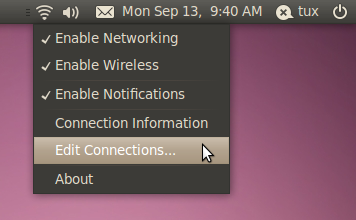
\includegraphics[width=8cm]{labs/kernel-module-environment/network-config-1.png}
\end{center}

Select the new wired network connection:

\begin{center}
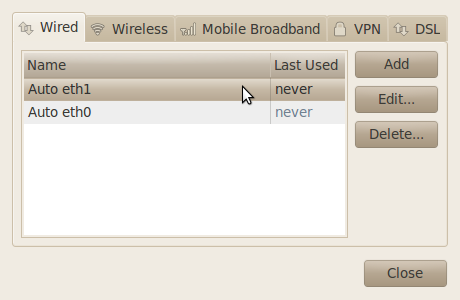
\includegraphics[width=8cm]{labs/kernel-module-environment/network-config-2.png}
\end{center}

In the \code{IPv4 Settings} tab, make the interface use a static IP
address, like \code{192.168.0.1} (of course, make sure that this address
belongs to a separate network segment from the one of the main company
network):

\begin{center}
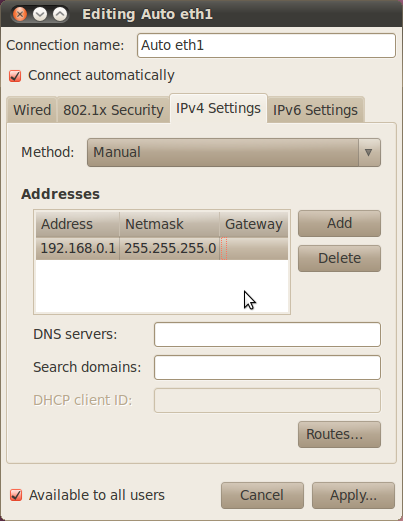
\includegraphics[width=8cm]{labs/kernel-module-environment/network-config-3.png}
\end{center}

Now, configure the network on the board in U-Boot by setting the
\code{ipaddr} and \code{serverip} environment variables:

\begin{verbatim}
setenv ipaddr 192.168.0.100
setenv serverip 192.168.0.1
\end{verbatim}

In case the board was previously configured in a different way, we
also turn off automatic booting after commands that can be used to
copy a kernel to RAM:

\begin{verbatim}
setenv autostart no
\end{verbatim}

To make these settings permanent, save the environment:

\begin{verbatim}
saveenv
\end{verbatim}

You can then test the TFTP connection. First, put a small text file in
the directory exported through TFTP on your development
workstation. Then, from U-Boot, do:

\begin{verbatim}
tftp 0x21000000 textfile.txt
\end{verbatim}

This should download the file \code{textfile.txt} from your development
workstation into the board's memory at location \code{0x21000000} (this
location is part of the board DRAM). You can verify that the download
was successful by dumping the contents of the memory:

\begin{verbatim}
md 0x21000000
\end{verbatim}

\section{Boot the system}

First, boot the board to the U-Boot prompt.  Before booting the
kernel, we need to tell it that the root filesystem should be mounted
over NFS, by setting some kernel parameters.  Use the following U-Boot
command to do so (in just 1 line):

\scriptsize
\begin{verbatim}
setenv bootargs root=/dev/nfs ip=192.168.0.100
  nfsroot=192.168.0.1:/home/<user>/felabs/linux/modules/nfsroot
\end{verbatim}
\normalsize

Of course, you need to adapt the IP addresses to your exact network
setup. Save the environment variables (with \code{saveenv}).  Now, download
the kernel image through \code{tftp}:

\begin{verbatim}
tftp 0x21000000 uImage
\end{verbatim}

Now, boot your kernel:

\begin{verbatim}
bootm 0x21000000
\end{verbatim}

If everything goes right, you should reach a shell prompt. Otherwise,
check your setup or ask your instructor for details.

If the kernel fails to mount the NFS filesystem, look carefully at the
error messages in the console. If this doesn't give any clue, you can
also have a look at the NFS server logs in \code{/var/log/syslog}.
